\documentclass{beamer}
\input{common.tex}

\title{Tutorium 14: Bytecode \& Wiederholung}
% \subtitle{}
\author{David Kaufmann}
\institute{Tutorium Programmierparadigmen am KIT}
\date{15. Februar 2023}

\begin{document}
\begin{frame}
	\titlepage
\end{frame}

\subsection{AST Erzeugung}

\begin{frame}{Aufgabe}
    Wir bauen den Parser von letzter Woche weiter...
    \begin{columns}
        \begin{column}{0.5 \textwidth}
            \begin{itemize}
                \item Zu jeder Kategorie eine Klasse
                \item Jeder Blatttyp und innerer Knoten ein Konstruktor
                \item Unterklassen für Kategorie sind Alternativen
                \item Baum soll links-assoziativ sein
            \end{itemize}
        \end{column}
        \begin{column}{0.5 \textwidth}
           $$(a+b+c)/a$$
           \begin{figure}
               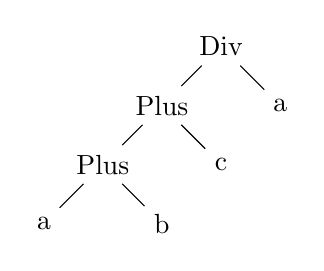
\begin{tikzpicture}[
                  level distance=7.5mm,
                  sibling distance=15mm
                ]
                  \node {Div}
                    child {
                      node {Plus}
                        child {
                          node {Plus}
                            child {node {a}}
                            child {node {b}}
                        }
                        child {node {c}}
                    }
                    child {node {a}}
                  ;
                \end{tikzpicture}
           \end{figure}
       \end{column}
    \end{columns}
\end{frame}

\begin{frame}{Aufgabe}
	\footnotesize
	\begin{align*}
		E     \to & \;\; T \;\; EList\\
		EList \to & \;\; \epsilon \mid \textrm{\texttt{+}} \;\; T \;\; EList \mid \textrm{\texttt{-}} \;\; T \;\; EList\\
		T     \to & \;\; F \;\; TList\\
		TList \to & \;\; \epsilon \mid \textrm{\texttt{*}} \;\; F \;\; TList \mid \textrm{\texttt{/}} \;\; F \;\; TList\\
		F \to & \;\; \textrm{\texttt{num}} \; | \; \textrm{\texttt{(}} \;\; E \;\; \textrm{\texttt{)}}
	\end{align*}
	\begin{itemize}
            \item Der Parser soll einen AST zurückgeben
		\item Verwendet die Klassen aus \texttt{./demos/compiler/Exp.java}
            \item Der Baum soll wie auf letzter Folie aussehen
	\end{itemize}
\end{frame}

\subsection{Semantische Analyse/Optimierung}

\begin{frame}{Semantische Analyse}
	\begin{itemize}
		\item PP beschäftigt sich (bis auf Typinferenz) nur kurz mit semantischer Analyse
		\item Typchecks/-inferenz, Namensanalyse
		\item $\leadsto$ weiterführende (Master-)Vorlesungen am IPD
	\end{itemize}
\end{frame}

\section{Java-Bytecode}

\begin{frame}{Umgekehrte Polnische Notation}
    Schreibweise für Ausdrücke, bei der zuerst die Operanden und dann die auszuführende Operation angegeben wird. 

    Ist die natürliche Darstellung für Stackmaschinen
    \hspace{1cm}
    \begin{columns}
        \begin{column}{0.3 \textwidth}
            \begin{itemize}
                \item $2 * 3$
                \item $2 * 3 + 4$
                \item $7 + 3 * (3+2)$
            \end{itemize}
        \end{column}
        \begin{column}{0.3 \textwidth}
            \begin{itemize}
                \pause
                \item $2 \; 3 \; *$
                \pause
                \item $2 \; 3 \; * \; 4 \;+$
                \pause
                \item $7 \; 3 \; 3 \; 2 \; + \; * \; +$
            \end{itemize}
        \end{column}
    \end{columns}
\end{frame}


\begin{frame}{wichtige Befehle}
    \begin{itemize}
        \item \texttt{X\_const\_i}: läd Konstante für $i \in [-1,5]$ auf den Stack
        \item \texttt{bipush <i>}: läd Konstante für $i \in [-127,128]$
        \item \texttt{Xload <x>, Xstore <x>}: lesen/schreiben von lokalen Variablen (für Integer gibt es eigenen Opcode für $x \in [0,3]$)
        \item \texttt{Xmul, Xadd,...}: Arithmetik
    \end{itemize}
\end{frame}

\begin{frame}{Beispiel}
    \begin{columns}
        \begin{column}{0.55 \textwidth}
            \code{./code/bytecode/calc.java}
            \hspace{1cm}
            
            Variablen \texttt{x, y, z} in lokalen Variablen 1, 2, 3 gespeichert
        \end{column}
        
        \begin{column}{0.3 \textwidth}
        \pause
        \texttt{iload\_1\\iconst\_2\\iadd\\istore\_3\\iload\_1\\iconst\_3\\imul\\iload\_3\\iadd\\istore\_2}
        \end{column}
    \end{columns}
\end{frame}

\begin{frame}{Sprünge}
    \begin{itemize}
        \item \texttt{goto label}: unbedingter Sprung
        \item \texttt{if\_icmpOP label}: bedingter Sprung, der die ersten beiden Integer auf dem Stack vergleicht 
        \item \texttt{ifOP label}: bedingter Sprung, der erstes Stackelement mit 0 vergleicht
        \item \texttt{ireturn}: gibt einen Integer zurück
    \end{itemize}
    OP $\in \{\texttt{eq, ge, gt, le, lt}\}$
\end{frame}

\begin{frame}{Beispiel}
    \begin{columns}
        \begin{column}{0.60 \textwidth}
            \code{./code/bytecode/fibs.java}
        \end{column}
        \begin{column}{0.4 \textwidth}
            \scriptsize
            \texttt{iconst\_1\\istore\_2\\iconst\_1\\istore\_3\\loop\_begin:\\iinc 1 1\\
            iload\_1\\ifle after\_loop\\iload\_2\\iload\_3\\iadd\\istore\_4\\iload\_2\\istore\_3
            iload 4\\istore\_2\\goto loop\_begin\\after\_loop:\\iload\_2\\ireturn}
        \end{column}
    \end{columns}
\end{frame}

\begin{frame}{Kurzauswertung}
    Bei \&\& und $||$ Kurzauswertung beachten!

    Löst man über ein weiteres label, zu dem man nur springt, wenn noch nicht entschieden

    Schreibt den Bytecode für:

    \texttt{if (a == 0 \&\& b == a + 1)}

    \pause

    Für Negation einfach Label vertauschen
\end{frame}

\begin{frame}{Arbeiten mit Klassen und Objekten}
    \begin{itemize}
        \item this kann mit \texttt{aload\_0} geladen werden
        \item \texttt{invokevirtual \#dest}: ruft in dest spezifizierte Methode auf
        \item \texttt{putfield name:type}: schreibt Wert von Typ type in Klassenvariable mit Name name. Auf dem Stack müssen der Wert und die Objectreferenz liegen
    \end{itemize}
\end{frame}

\begin{frame}{Arrays}
    \begin{itemize}
        \item \texttt{newarray type}: erzeugt ein neues Array. Verwendet das oberste Element auf dem Stack als Länge
        \item \texttt{astore}: speichern einer Referenz (z.B. Array)
        \item \texttt{iaload}: läd Wert von Index aus Array. Stack muss von oben belegt sein mit: Index, Array Referenz.
        \item \texttt{iastore}: speichert Integer an Index in Array. Stack muss aussehen von oben: Wert, Index, Array Referenz
    \end{itemize}
\end{frame}

\section{Klausuraufgabe SS17 Aufgabe 12}

\section{Evaluation}

\begin{frame}{Wiederholung}
    \begin{itemize}
        \item Haskell: SS17 Nr. 1, 2
        \item Prolog: ÜB 7 Nr. 3
        \item $\beta$-Reduktion: SS17 Nr. 6a
        \item Lambda: SS18 Nr. 4
        \item Unifikation: SS17 Nr. 4
        \item Typinferenz: ÜB 9 Nr. 4
        \item MPI: SS17 Nr. 7
        \item Java: WS1718 Nr. 7
        \item Design By Contract: WS1718 Nr. 8
        \item Parser: SS20 Nr. 10
        \item Bytecode: WS2021 Nr. 8
    \end{itemize}
\end{frame}
\section{Ende}

\begin{frame}{Letzte Folie}
  \begin{itemize}
    \item ÜB-Korrekturen: Blatt 13 korrigiere ich noch
    \item Klausur: 31.03.2023, 11:30
    \item Tutoriumsfolien, -code, etc.: \href{https://github.com/KaufmannDavid/propa-tut}{github.com/KaufmannDavid/propa-tut}
    \item Fragen auch gerne an \texttt{david.kaufmann@student.kit.edu} :)
  \end{itemize}

  \vfill

  Danke fürs Kommen und eine erfolgreiche Prüfungsphase!
\end{frame}
\end{document}